\documentclass[14pt, fleqn, xcolor={dvipsnames, table}]{beamer}
\usepackage[T2A]{fontenc}
\usepackage[utf8]{inputenc}
\usepackage[english,russian]{babel}
\usepackage{amssymb,amsfonts,amsmath,mathtext}
\usepackage{cite,enumerate,float,indentfirst}
\usepackage{cancel}
\usepackage{graphicx}
\usepackage{animate}
\usepackage{ulem}

\usepackage{tikz}
% \usepackage{enumitem}
\usetikzlibrary{shadows}

% \usepackage{enumitem}
% \setitemize{label=\usebeamerfont*{itemize item}%
%   \usebeamercolor[fg]{itemize item}
%   \usebeamertemplate{itemize item}}

\graphicspath{{images/}}

\usetheme{Madrid}
\usecolortheme{seahorse}
\renewcommand{\CancelColor}{\color{red}}

\setbeamercolor{footline}{fg=Blue!50}
\setbeamertemplate{footline}{
  \leavevmode%
  \hbox{%
  \begin{beamercolorbox}[wd=.333333\paperwidth,ht=2.25ex,dp=1ex,center]{}%
    И. Кураленок
  \end{beamercolorbox}%
  \begin{beamercolorbox}[wd=.333333\paperwidth,ht=2.25ex,dp=1ex,center]{}%
    Санкт-Петербург, 2017
  \end{beamercolorbox}%
  \begin{beamercolorbox}[wd=.333333\paperwidth,ht=2.25ex,dp=1ex,right]{}%
  Стр. \insertframenumber{} из \inserttotalframenumber \hspace*{2ex}
  \end{beamercolorbox}}%
  \vskip0pt%
}
\newcommand\indentdisplays[1]{%
     \everydisplay{\addtolength\displayindent{#1}%
     \addtolength\displaywidth{-#1}}}
\newcommand{\itemi}{\item[\checkmark]}

\newenvironment{mydescription}[1]
  {\begin{list}{}%  
   {\renewcommand\makelabel[1]{\color{blue}##1:\hfill}%
   \settowidth\labelwidth{\makelabel{#1}}%
   \setlength\leftmargin{\labelwidth}
   \addtolength\leftmargin{\labelsep}}}
  {\end{list}}

\title{Генеративный подход к обучению на последовательностях}
\author[]{\small{%
И.~Куралёнок}}
\date{}
\begin{document}

\begin{frame}
\maketitle
\small
\begin{center}
\vspace{-60pt}
\vspace{80pt}
\footnotesize СПб, 2017
\end{center}
\end{frame}

\section{Постановка задачи}

\begin{frame}{Чему мы учимся на последовательностях}
$$
s = \{w_i\}_1^{T_s}, w_i \in \mathcal{A}
$$
\begin{description}
  \item[Классификации:] есть примеры $s$ и правильные классы на них $y_i \in \{1,\ldots,k\}$
  \item[Сегментации:] в строке $s$ в момент времени $t_s$ что-то идет не так, хотим как можно лучше предсказать $t_s$
  \item[Генерация:] предсказываем следующий символ
  \item[Маркировка:] каждому элементу ставим в соответствие маркер $y_i \in \{1,\ldots,k\}$
\end{description}
\uncover<1->{$\Rightarrow$ Все можно свести к маркировке!}
\end{frame}

\begin{frame}{Преобразования алфавитов}
\begin{itemize}
  \item $w \in \mathbb{R}$ \uncover<2->{$\Rightarrow$ ``порежем'' область значений $w$ (например медианами), получим обычный алфавит.}
  \item $w \in \mathbb{R}^n$ \uncover<3->{$\Rightarrow$ проделаем предыдущий фокус и запишем в алфавит все комбинации букв компонент.}
  \item Алфавиты можно уменьшать \uncover<4->{$\Rightarrow$ закодируем символы в $\mathcal{A}_0 = \{0,1\}$.}
  \item Алфавиты можно увеличивать \uncover<5->{$\Rightarrow$ выделим подпоследовательности, скажем что это и есть новый алфавит.}
\end{itemize}
\end{frame}

\begin{frame}{Общая генеративная схема}
Сегодня мы будем подходить к проблеме маркировки следующим образом:
\begin{enumerate}
  \item Пусть $\Omega = \{1,\ldots,k\}$
  \item $X_t: \Omega \to \mathbb{R}^+$
  \item Будем искать такие последовательности $X_t$, которые будут доставлять в максимум:
  $$
    \sum_{t=1}^{T} \log {X_t(y_t) \over \sum_y X_t(y)}
  $$
\end{enumerate}
\end{frame}

\section{Наивные методы}

\begin{frame}{Наивный подход I}{\uncover<2->{n-gram}}
Будем считать, что $X_t$ определяется только текущим символом:
$$
X_t(y) = X_{w_t}(y)
$$

\end{frame}

\begin{frame}{Наивный подход II}{\uncover<2->{Bag of words}}
Будем рассматривать всю предыдущую историю как множество:
$$X_t = X: \Omega \times \mathbb{R}^{|\mathcal{A}|} \to \mathbb{R}$$
При этом, задав категории $y$ целевой развесовкой в $\mathbb{R}^{|\mathcal{A}|}$ $X$ можно строить так:
$$X_t = y^T TF(s_t)$$
\end{frame}

\section{Скрытые марковские цепи}

\begin{frame}{Hidden Markov Model}
\begin{definition}[HMM]
Пускай $x_t \in \{\xi_i\}_1^p$, где $\xi_i$---простая случайная величина над $\Omega$, заданная строкой матрицы $A$.
Переходы от $x_t$ к $x_{t+1}$ случайны и заданы матрицей переходов $B$. Тогда получившийся процесс называется скрытой марковской моделью c параметрами $A$ и $B$.
\end{definition}
$\Rightarrow$ кажется, такую штуку можно использовать для нашей задачи, вопрос только в том откуда начать и как пойти, так как это почти электрон :)
\end{frame}

\begin{frame}{Viterbi}
HMM можно учить исходя из $X_t = x_t$:
\begin{enumerate}
  \item  C помощью Байеса можно получить наиболее вероятный маршрут $r(s)$, генерирующий данный пример:
$$\begin{array}{l}
p_{ti} = b_{iw_t} \sum_k p_{{t - 1}k} a_{ik} \\
r(s)_t = \arg \max_i p_{ti}
\end{array}$$
  \item Будем считать, что этот маршрут и наблюдался (expectation step)
  \item Подвинем веса $A$ и $B$ в соответствии с этим знанием (maximization step)
\end{enumerate}
\end{frame}

\subsection{Взад-назад алгоритм}

\begin{frame}{Как получить ответ от HMM}
Как у настоящего электрона, у HMM можно посчитать ожидание вместо одного генерирующего маршрута:
$$
X_t = \sum_\xi \xi \sum_r P(r|s,A,B) I\{x_{rt} = \xi\}
$$
Тут есть только одна проблема, $X_t$ считается довольно долго из-за того что маршрутов -- трилиарды.
\end{frame}

\begin{frame}{Взад-назад алгоритм}{Forward-Backward algorithm}
С помощью формулы Байеса легко показать, что:

$$\begin{array}{l}
P(X_t = \xi| s, A, B) = \sum_r P(r|s,A,B) I\{x_{rt} = \xi\} \sim f_{\xi t} b_{\xi t} \\
f_{t}  = f_{t-1} A\ diag(b_{w_t}) \\
b_{t}  = b_{t+1} A\ diag(b_{w_{t+1}})
\end{array}$$
\end{frame}


\begin{frame}{Baum-Welch}
Попробуем напрямую максимизировать:
$$\begin{array}{l}
(\hat{A}, \hat{B}) = \arg \max_{A,B} \sum_{t=1}^{T} \log {X_t(y_t) \over \sum_y X_t(y)} \\
X_t = \sum_\xi \xi P(X_t = \xi| s, A, B) = \\
P(X_t = \xi| s, A, B) = \sim f_{\xi t} b_{\xi t} \\
\end{array}$$
\small
\uncover<2->{Это не кажется простым занятием :)\\
Оказывается можно максимизировать не это, а делать такие шаги:
$$
(A_t, B_t) = \arg \max_{A,B} \sum_t P(w_t, y_t| A, B) \log P(w_t, y_t| A_{t-1}, B_{t-1})
$$
}
\end{frame}

\subsection{Анализ HMM}
\begin{frame}{Критика HMM}
\begin{itemize}
  \item Конечное количество состояний
  \item Каждое состояние приносит $|\Omega|$ параметров
  \item Непонятно как делать классификацию
\end{itemize}
\end{frame}

\section{Условные случайные поля}

\subsection{Random fields}

\begin{frame}{Случайные поля}
Это такое обобщение случайных процессов, которое позволяет индексировать случайные переменные любыми множествами. Например графами :).
\end{frame}

\begin{frame}{Conditional Random Fields}
\begin{enumerate}
  \item Хотим ограничить не количество состояний, а ввести зависимость состояний:
$$X_t = f(X_{t-1})$$
В этом случае обобщение будет строится не вокруг малого количества состояний, а на степени зависимости соседних состояний.
  \item Так как мы строим зависимость, можно использовать знание о $y_{t-1}$.
\end{enumerate}
\end{frame}

\begin{frame}{Преобразование состояния в CRF}
Введем функции $f$ и $g$, зависящие от соседей по графу. $f$---от перехода, $g$---от нода.
{\small
$$\begin{array}{c}
X_t(\lambda, \mu) =
\exp\left(\sum_{k,e} \lambda_k f_k(e, y|_e, w_t)
 + \sum_{k,v} \mu_k g_k(v, y|_v, w_t) \right)
\end{array}$$
}
Теперь количество параметров определяется количеством функций, а не состояний.
\end{frame}

\begin{frame}{Подбор параметров CRF}
Можно напрямую оптимизировать:
$$
(\hat{\lambda}, \hat{\mu}) = \arg \max_{\lambda, \mu} \sum_s \sum_{t=1}^{T_s} \log {X_t(y_t, x, \lambda, \mu) \over \sum_y X_t(y, x, \lambda, \mu)}
$$
\begin{itemize}
  \item Целевая функция {\bf выпукла}
  \item Оригинально оптимизируется с помощью IIS\footnote{Improved Iterative Scaling, Della Pietra et. al. 1997} или аналогом Baum-Welch
  \item Кажется, что можно простым SGD, или даже GD
\end{itemize}
\end{frame}

\begin{frame}{Критика CRF}
\begin{itemize}
  \item Надо подбирать функции исходя из доменной области
  \item Эффективность работы существенно меняется от набора функций
\end{itemize}
\end{frame}

\section{LSTM}

\subsection{RNN}
\begin{frame}{Рекурентные нейронные сети}
Когда думать не хочется, можно воспользоваться сетями :).
\begin{center}
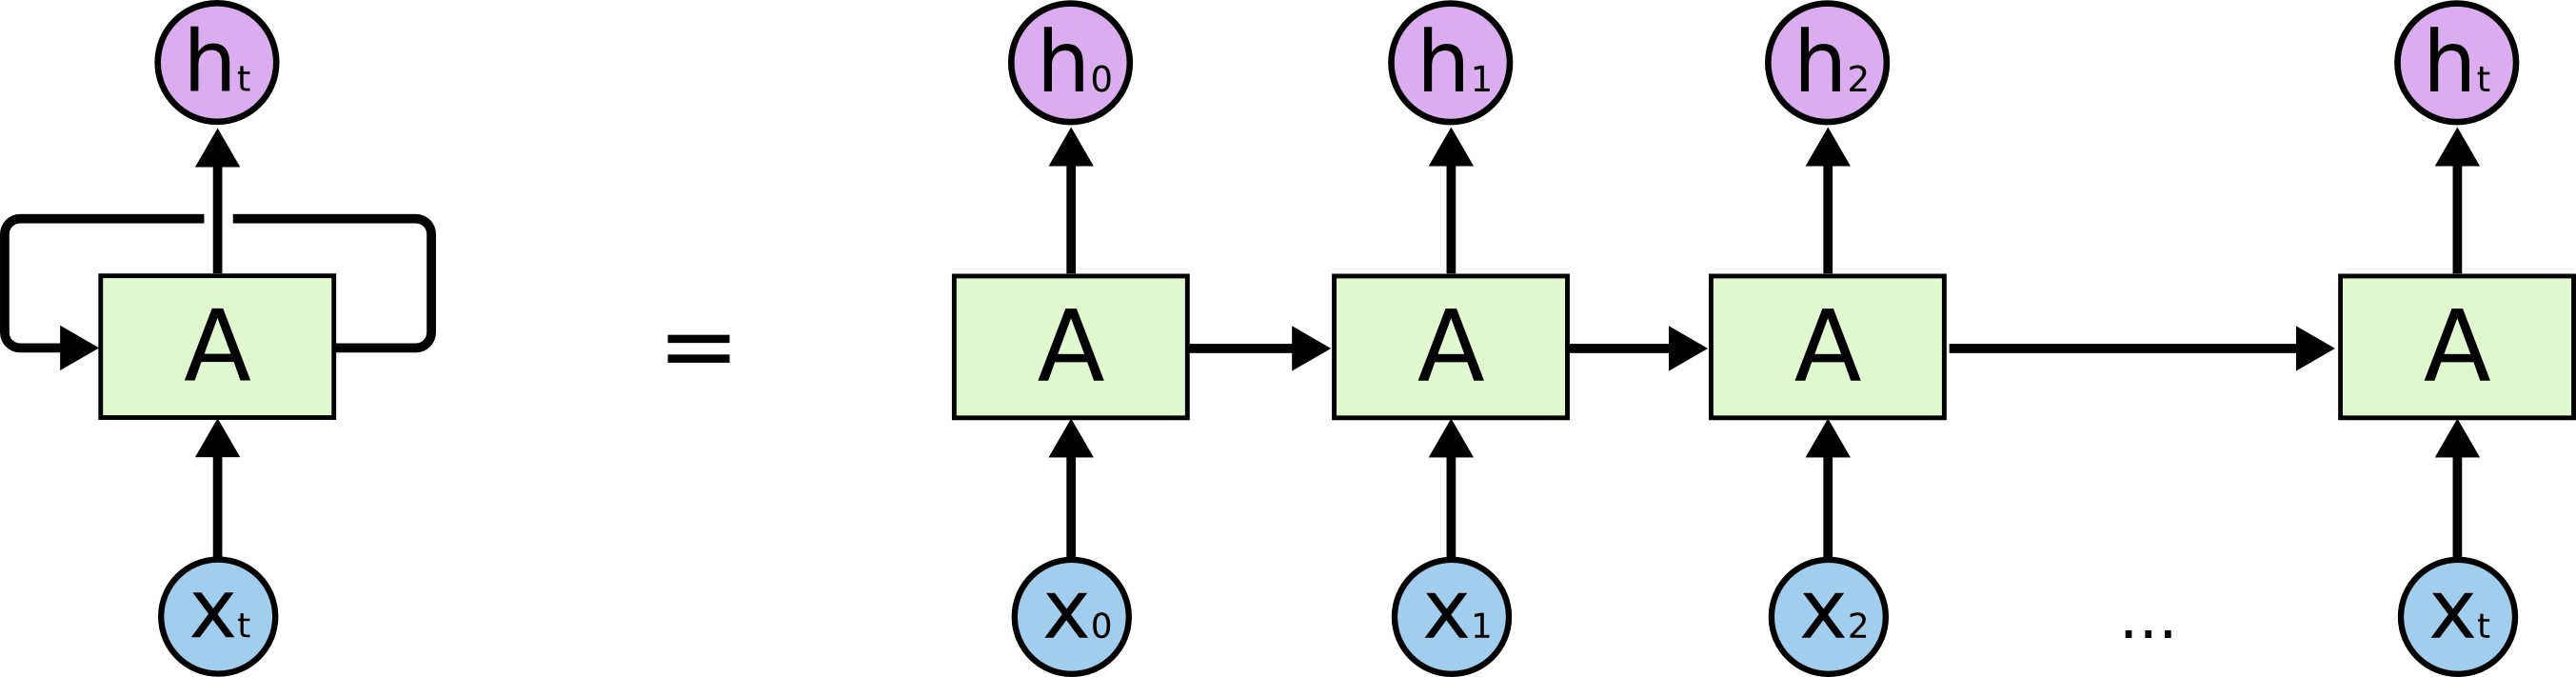
\includegraphics[width=0.7\textwidth]{RNN-unrolled.png}\footnote{Красивые картинки взяты тут: http://colah.github.io/posts/2015-08-Understanding-LSTMs/}
\end{center}
В нашем случае рекурентными. Назначим $X_t$ выходным вектором $h$.
\end{frame}

\begin{frame}{Особенности обучения RNN}
Можно использовать back propagation!

$$
\frac{\partial T}{\partial \beta} = \sum_l \frac{\partial T}{\partial s_l} \frac{\partial s_l}{\partial \beta}
$$
К сожалению, такая сумма очень шумная (из-за наличия дополнительных входных сигналов) + сигнал быстро затухает.
\end{frame}
\subsection{LSTM}

\begin{frame}{Long-Short Term Memory}
Hochreiter \& Schmidhuber в 1997 г. придумали механизм сохранения сигнала:
\begin{center}
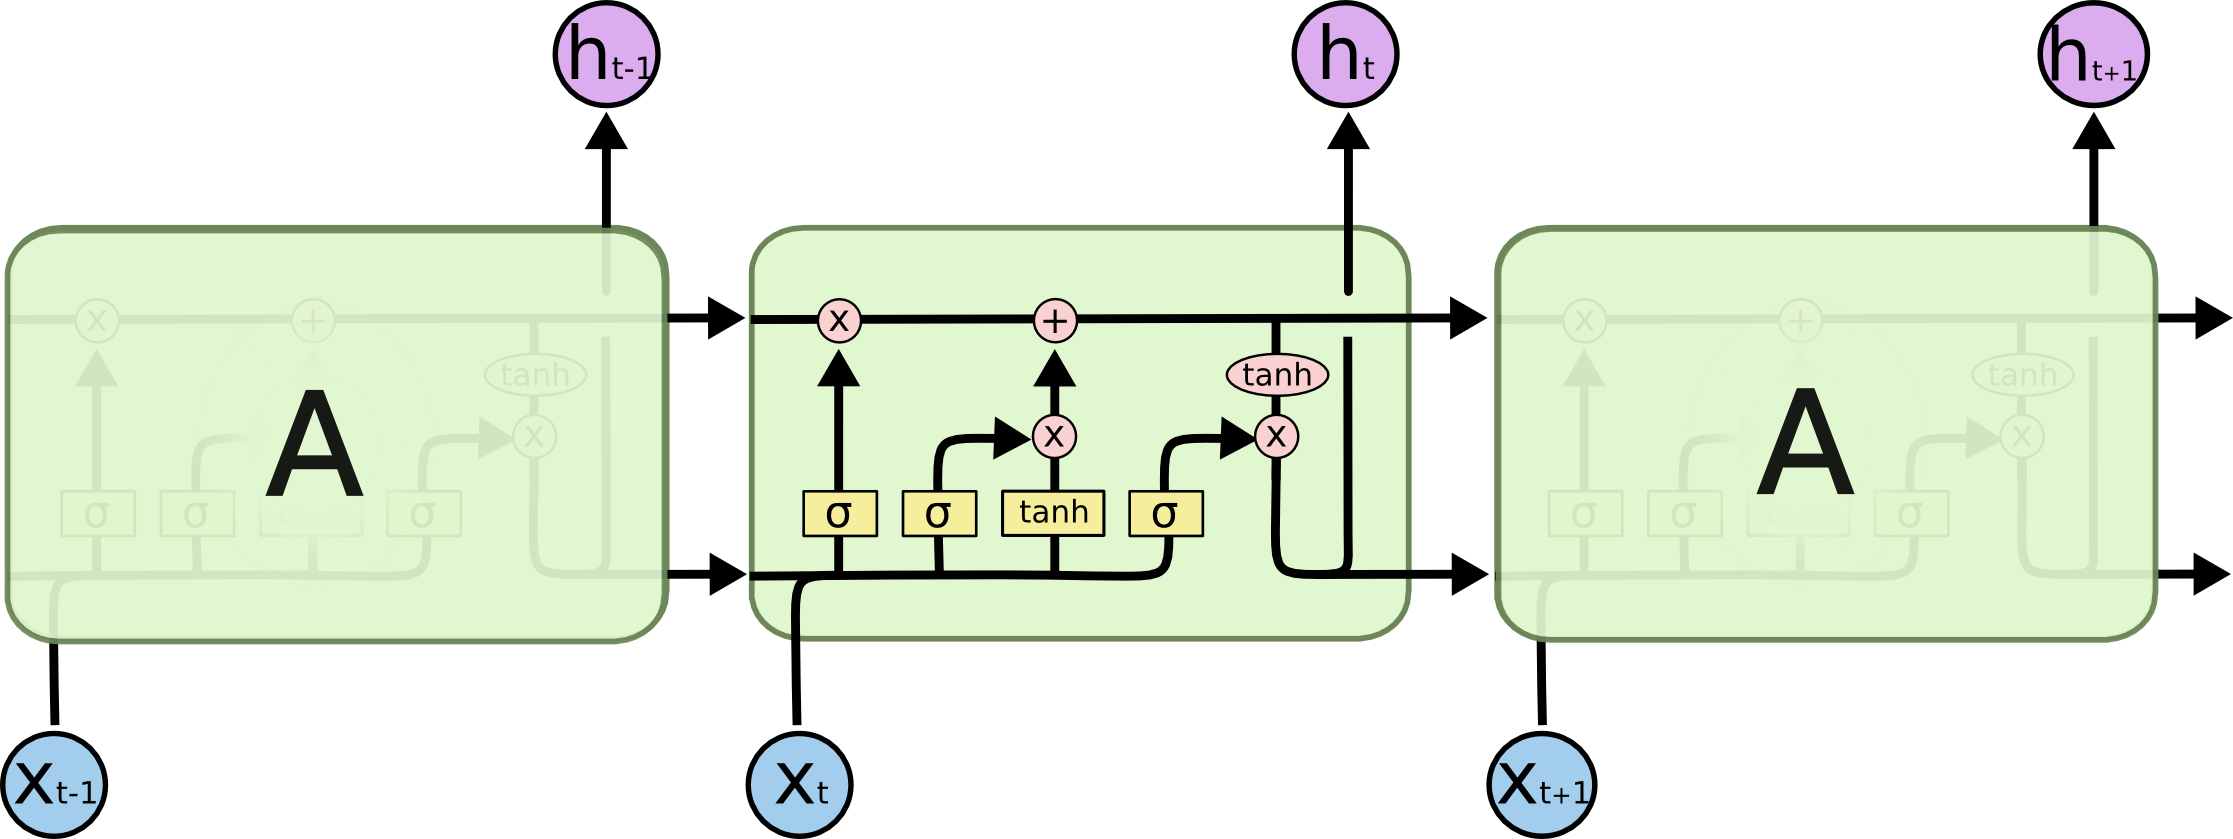
\includegraphics[width=0.7\textwidth]{LSTM3-chain.png}
\end{center}

\end{frame}

\section{Выводы}

\begin{frame}{Что мы сегодня узнали}
\begin{itemize}
  \item Есть такая задача, работать с последовательностями
  \item Ее можно решать генеративными моделями на случайных процессах
  \item Механизм моделирования усложнялся со временем
  \item Из-за подхода сверху-вниз рассмотренные методики до сих пор эффективны во многих доменных областях
\end{itemize}
\end{frame}

\end{document}
